The methodology adopted in this study consists of a structured pipeline for the automatic classification of ISUP grades in prostate histopathological images, as illustrated in Figure~\ref{fig:methodology}. The PANDA dataset is first acquired and preprocessed, then split into training and test sets. Next, noise-reduction filtering is applied exclusively to the training set, with the goal of removing potentially inconclusive images that could compromise the models' learning. After this step, whole-slide images are fragmented into patches, reducing spatial dimensionality and making training computationally more efficient. In the modeling phase, different individual classifiers are trained using distinct learning strategies. Finally, an ensemble approach is used to combine the predictions of these models, yielding a more robust and stable solution.

\begin{figure}[h]
	\centering
	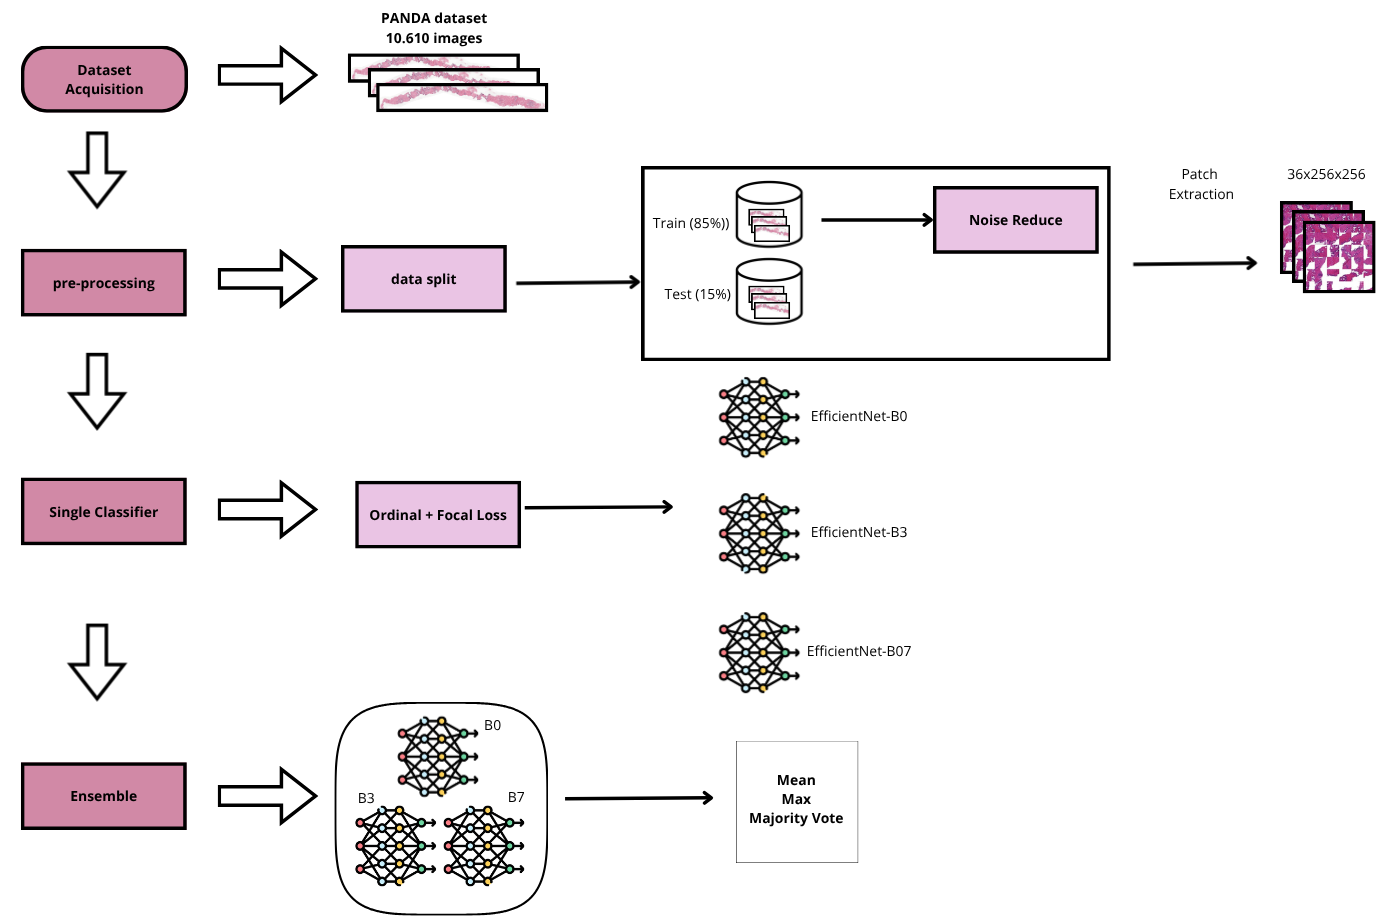
\includegraphics[width=1\linewidth]{images/methodology}
	\caption{proposed method}
	\label{fig:methodology}
\end{figure}


\subsection{Dataset Acquisition}
\label{subsec:data-acquisition}
We used the Prostate Cancer Grade Assessment (PANDA) dataset~\cite{ref-panda2020}, which consists of 10,616 whole-slide images (WSIs) of high-resolution (20×) digitized prostate biopsies. Each image is annotated according to the ISUP grading system (0–5), where grade 0 indicates the absence of malignancy, and grades 1-5 represent increasing levels of tumor aggressiveness.

The Table~\ref{tab:dist_classes} presents the class distribution of the dataset. A significant class imbalance is observed, with a predominance of class 0 (approximately 27\%). In contrast, the classes associated with more advanced clinical grades (ISUP 4 and 5) each represent less than 12\% of the total.

The PANDA images originate from two distinct medical centers: Radboud University Medical Center and Karolinska Institutet. According to the authors~\cite{ref-panda2020}, the slides from Radboud were annotated by trained students, whereas experienced pathologists labeled those from Karolinska. This heterogeneity introduces inter-institutional variability in the annotations. In addition, the public dataset contains various forms of noise, including annotations and pen markings near tumor regions, which can adversely affect model training quality.

\begin{table*}[!ht]
	\centering
	\begin{tabular*}{\textwidth}{@{\extracolsep\fill}llll@{}}
		\toprule
		\textbf{ISUP Grade} & \textbf{Karolinska} & \textbf{Radboud} & \textbf{Total} \\
		\midrule
		0 & 1,520 (27.9\%) & 1,372 (26.6\%) & 2,892 (27.24\%) \\
		1 & 1,404 (25.7\%) & 1,262 (24.4\%) & 2,666 (25.11\%) \\
		2 & 690 (12.6\%) & 653 (12.7\%) & 1,343 (12.65\%) \\
		3 & 635 (11.6\%) & 607 (11.8\%) & 1,242 (11.70\%) \\
		4 & 641 (11.7\%) & 608 (11.8\%) & 1,249 (11.77\%) \\
		5 & 566 (10.3\%) & 658 (12.7\%) & 1,224 (11.53\%) \\
		\midrule
		\textbf{Total} & \textbf{5,456 (51.3\%)} & \textbf{5,160 (48.7\%)} & \textbf{10,616 (100\%)} \\
		\bottomrule
	\end{tabular*}
	\begin{tablenotes}
		\item {\it Source}: Data derived from the PANDA Challenge dataset (2020).
	\end{tablenotes}
	\caption{Characteristics of the PANDA dataset used in this study.\label{tab:dist_classes}}
\end{table*}


\subsection{Preprocessing}
\label{subsec:preprocessing}

The preprocessing pipeline was structured in a sequential manner to ensure evaluation integrity and sample quality. The process begins with a stratified data split, followed by an uncertainty-based (entropy) filtering step to remove noisy instances. Finally, to address the high dimensionality of whole-slide images and to increase the variability of the training set, patch extraction and data augmentation techniques are applied.

\subsubsection{Data Partitioning and Noise Filtering}
\label{subsubsec:partitioning-filtering}
Initially, a stratified split of the dataset was performed to preserve the original class distribution. Of the total images, 15\% were reserved for the final test set, while the remaining 85\% comprised the development set.

Considering the presence of noisy labels, as illustrated in Figure~\ref{fig:noise}, which shows an image with visible pen markings, and the high complexity involved in discriminating specific samples (Section~\ref{subsec:data-acquisition}), a filtering mechanism based on Shannon entropy was implemented. This metric, widely used in Information Theory and Artificial Intelligence applications, allows quantifying the degree of uncertainty associated with the model predictions~\cite{ali2023entropy}.

\begin{figure}[!htb]
	\centering
	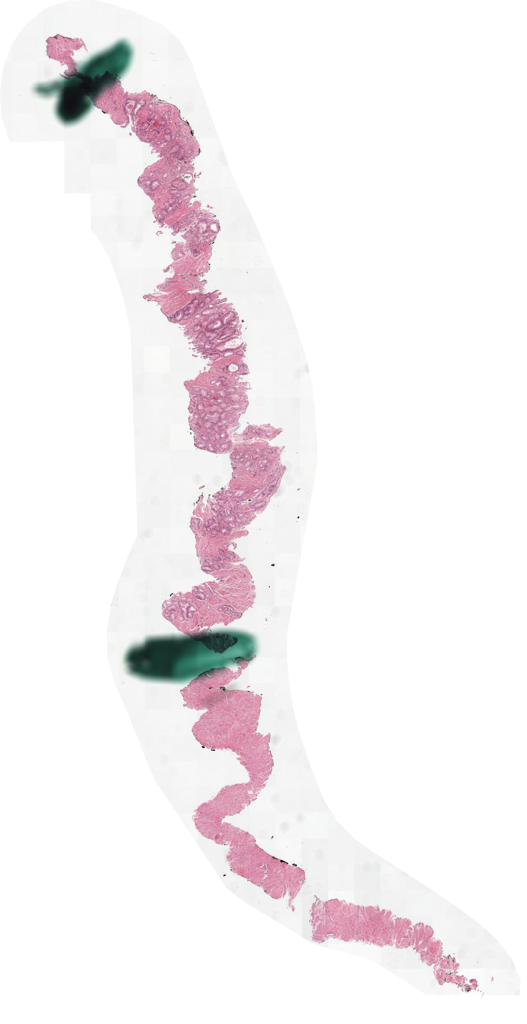
\includegraphics[width=0.4\textwidth, height=0.3\textheight]{images/slide_thumbnail.png}
	\caption{Example of an image containing noise.}
	\label{fig:noise}
\end{figure}

For each instance, the model generates a probability distribution over the $K$ classes, denoted by $p = [p_1, \ldots, p_K]$. The entropy is then defined as:

\begin{equation}
	H(p) = -\sum_{i=1}^{K} p_i \log(p_i),
\end{equation}



\noindent where low values indicate higher model confidence, as the probability distribution is concentrated in a few classes, in contrast, higher values are associated with more uniform distributions, reflecting greater predictive uncertainty and suggesting that the sample may be ambiguous, noisy, or of low quality. Therefore, entropy was adopted as a systematic indicator of sample difficulty and was applied exclusively to the development set.

The filtering process was conducted in three stages. First, an EfficientNet-B0 model pretrained on ImageNet~\cite{russakovsky2015imagenet} was used to estimate the probability distributions of all samples in the development set, from which entropy values were computed. Next, the impact of removing the highest-entropy instances was evaluated by testing thresholds for excluding the top 10\%, 5\%, and 2\% most uncertain examples. Finally, the 2\% threshold was selected as it provided the best balance between noise reduction and preservation of the available data volume.

After removing the noisy samples, the development set was stratified into 80\% for training and 20\% for validation. Table~\ref{tab:dataset-filter} presents the data distribution before and after filtering.

\begin{table}[!ht]
	\centering
	\begin{tabular*}{\columnwidth}{@{\extracolsep\fill}lrc@{}}
		\toprule
		\textbf{Subset} & \textbf{\% of Total} & \textbf{No. of Images} \\ 
		\midrule
		Test & 15\% & 1,590 \\
		\midrule
		\multicolumn{2}{l}{\textit{Development Set (Pre-Filtering)}} & \textit{9,024} \\
		\multicolumn{2}{l}{\textit{Development Set (Post-Filtering)}} & \textit{8,844} \\
		\midrule
		Training & $\approx$68\% & 7,075 \\
		Validation & $\approx$17\% & 1,769 \\ 
		\midrule
		\textbf{Total Used} & \textbf{100\%} & \textbf{10,434} \\ 
		\bottomrule
	\end{tabular*}
	\caption{Dataset distribution after noise filtering (2\% threshold).\label{tab:dataset-filter}}
\end{table}


\subsubsection{Patch extraction}
Given the size of the WSIs and the presence of non-informative areas, a preprocessing step was applied to optimize computational resources while preserving regions relevant to diagnosis. Initially, fixed patches of 256 × 256 pixels were extracted, selected based on empirical criteria for mean intensity and saturation in the RGB channels, to eliminate background regions, artifacts, and areas lacking diagnostic staining. Figure~\ref{fig:origin-tiles} illustrates the original histopathological image used as the basis for patch extraction and the resulting composite image after patch extraction and rearrangement, providing a visual understanding of the process.

\begin{figure}[!htb]
	\centering
	\subfloat[\centering Original]{{
\includegraphics[width=0.15\textwidth, height=0.24\textheight]{images/original.png} }}%
	\qquad
	\subfloat[\centering Patched image]{{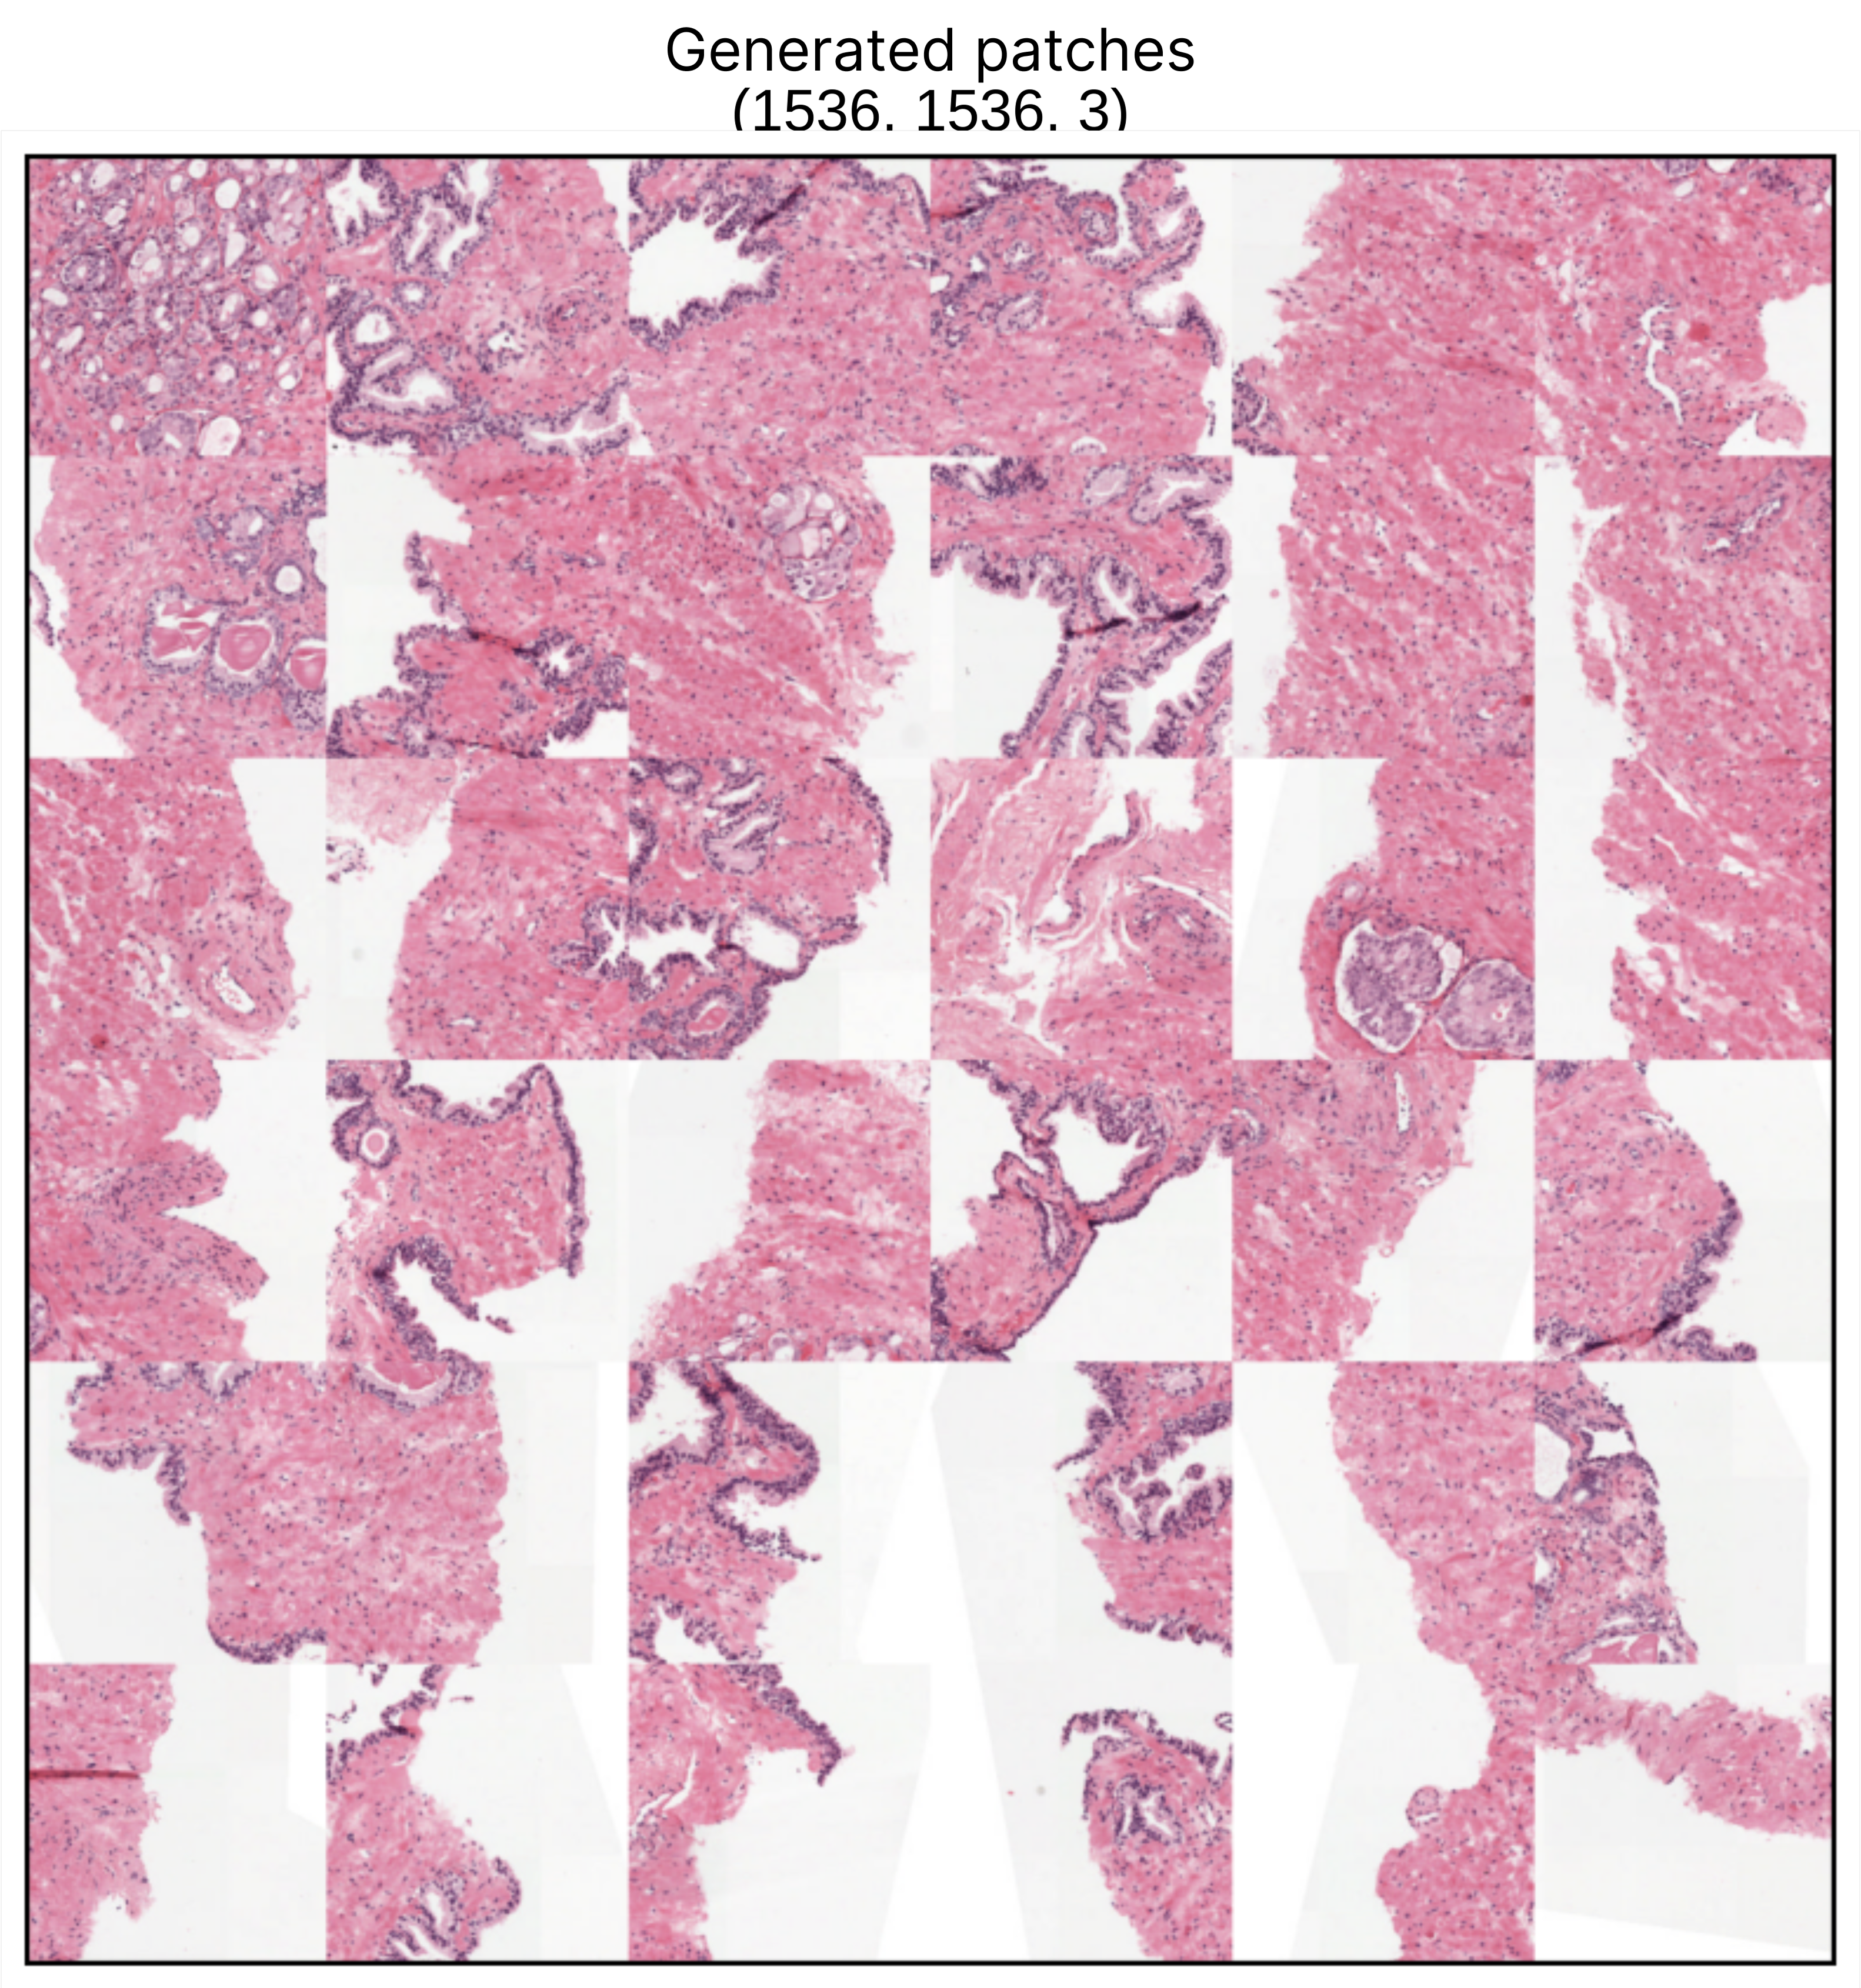
\includegraphics[width=0.4\textwidth,height=0.24\textheight]{images/tiles.png} }}%
	\caption{Original histopathological image (a) and composite image after patch extraction and rearrangement (b).}
	\label{fig:origin-tiles}
\end{figure}

For each slide, 36 patches were extracted, a number defined through preliminary experiments that evaluated the impact of the number of regions on morphological representativeness and computational feasibility. To support this choice, three configurations were compared: 25, 36, and 49 patches per slide, as illustrated in Figure~\ref{fig:tiles-original}.

\begin{figure}[!htb]
	\centering
	
\includegraphics[width=0.9\textwidth]{images/tiles-original.png}
	%
	\caption{Representation of patch extraction with different quantities. The image shows three examples: (a) with 25 patches, (b) with 36 patches, and (c) with 49 patches, displayed from left to right.}
	\label{fig:tiles-original}%
\end{figure}

The extraction with 25 patches produced a compact composition, thereby generating fewer data to analyze, which may reduce computational demands during model training and validation. However, this configuration limits slide coverage, resulting in a significant loss of morphologically relevant patterns for classification. In contrast, extracting 49 patches expanded the analyzed area but increased computational and storage costs, and included many empty or redundant regions that may negatively affect processing efficiency. Moreover, including peripheral areas with low discriminative content can compromise representation quality by diluting or saturating important features.

Thus, the intermediate configuration with 36 patches provides an appropriate balance between morphological coverage and computational efficiency, capturing most of the relevant information without overloading the image with irrelevant regions. For this reason, this configuration was adopted as the standard in this work. After extraction, the patches were rearranged and concatenated into a single composite image. Unlike approaches that preserve the original spatial distribution, in this study the patches were ordered by the amount of morphological information they contained, estimated from intensity and saturation measures in the RGB channels.

\subsection{Single Classifiers}

In the initial phase of the experiments, the EfficientNet-B0 model was adopted as a reference for hyperparameter optimization. A baseline was first established using the Binary Cross-Entropy (BCE) loss function. This choice was motivated by the nature of the problem, considering that a single slide may exhibit multiple lesion grades.
During the baseline training, several strategies were evaluated, including Stochastic Weight Averaging (SWA), Test Time Augmentation (TTA), and variations in learning rate, number of epochs, optimizers, and color spaces. Across all experiments, the model exhibited early convergence (between epochs 7 and 10), followed by overfitting, as illustrated in Figure~\ref{fig:loss_BCE}.

\begin{figure}[!htb]
	\centering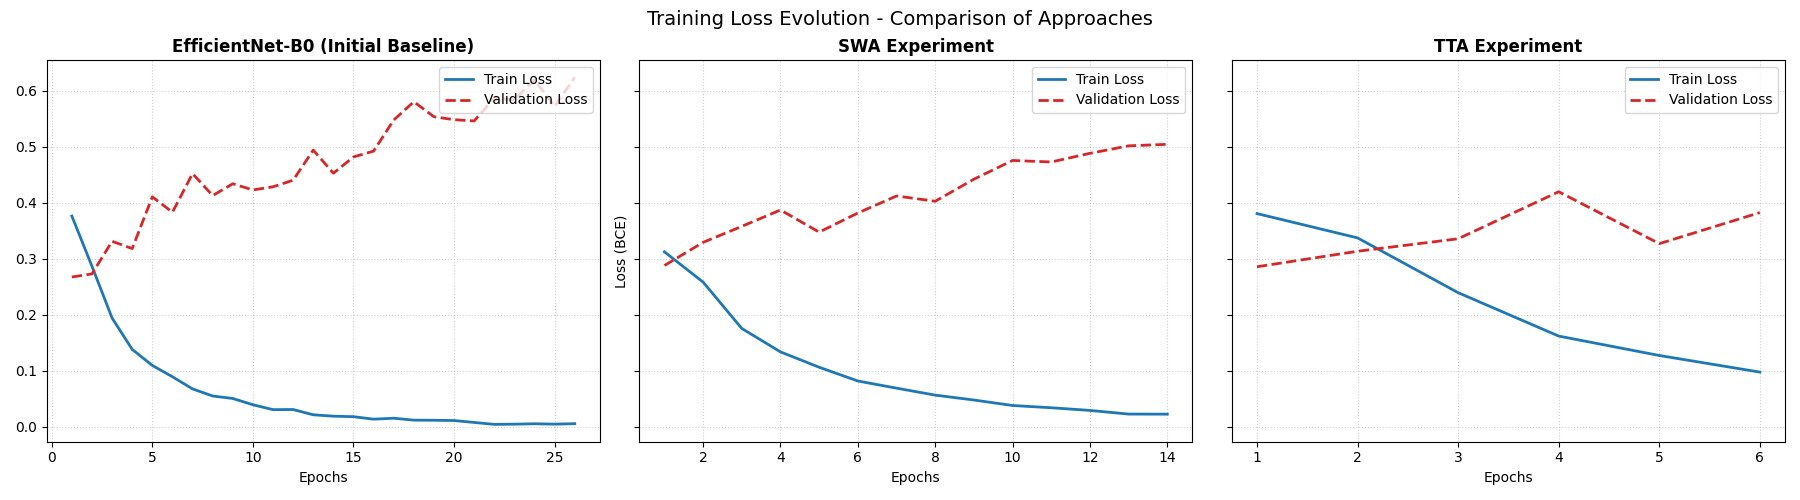
\includegraphics[width=1\textwidth]{images/overfitting.png}
	\caption{Baseline model training evolution curve.}
	\label{fig:loss_BCE}
\end{figure}

The main hypothesis for this behavior is that the BCE loss treats classes as independent nominal entities. Consequently, the model is penalized equally for confusing ISUP 0 with ISUP 1 (a minor clinical error) and for confusing ISUP 0 with ISUP 5 (a severe clinical error). This limitation motivated the adoption of an ordinal regression–based approach.

The proposed architecture employs ordinal regression to model the continuous and hierarchical nature of the ISUP grading system. The $K$-class problem is reformulated as $K-1$ binary classification tasks, where the $k$-th output corresponds to the conditional probability $P(y > k)$. The target labels ($y$) are mapped to ordinal vectors $V = [v_0, \ldots, v_{K-2}]$, formally defined as:

\[
v_k =
\begin{cases}
	1, & \text{if } y > k \\
	0, & \text{otherwise}
\end{cases}
\]

Thus, an ISUP grade 3 is encoded as $[1, 1, 1, 0, 0]$.

This structure imposes a monotonicity constraint on the labels, preventing logically inconsistent configurations and enabling the model to capture the hierarchical relationships among cancer severity grades. Subsequently, the Focal Loss technique~\cite{lin2017focal} was integrated into the ordinal approach to mitigate class imbalance. Focal Loss reshapes the standard cross-entropy loss by introducing a modulation factor $(1 - p_t)^\gamma$, which reduces the relative weight of easy (well-classified) examples, thereby forcing the model to focus training on hard and misclassified samples.

Table~\ref{tab:baseline_config} presents the hyperparameters used for training the models.

\begin{table}[!ht]
	\centering
	\begin{tabular*}{\columnwidth}{@{\extracolsep\fill}llc@{}}
		\toprule
		\textbf{Configuration} & \textbf{Parameter} & \textbf{Value} \\
		\midrule
		Training & Initial learning rate & $3 \times 10^{-4}$ \\
		& Maximum epochs & 50 \\
		& Batch size & 3 \\
		& Early stopping (patience) & 7 \\
		& Warmup & 1 epoch (factor 2) \\
		& Scheduler & Cosine Annealing \\
		& Optimizer & Adam \\
		& Fine-tuning & 150 layers \\
		\midrule
		Regularization & Dropout & 0.6 \\
		& Data augmentation & Flip/Transpose ($p=0.5$) \\
		& Entropy filtering & Top 2\% removed \\
		\midrule
		Focal Loss & $\alpha$ (alpha) & [0.25, 0.35, 0.50, 0.70, 0.90] \\
		& $\gamma$ (gamma) & 2.0 \\
		\midrule
		Inference & Aggregation & Mean of predictions \\
		Architectures & Tested backbones & EfficientNet-B0/B3/B7 \\
		& Output classes & 6 \\
		\bottomrule
	\end{tabular*}
	\caption{Experiment configuration for the proposed approach.\label{tab:baseline_config}}
\end{table}



\subsection{Ensemble}
To maximize predictive performance, we adopted an ensemble composed of the EfficientNet-B0, B3, and B7 models. The literature supports this approach due to its greater robustness and generalization capabilities compared to using individual models~\cite{mian2024ensemble}. Different strategies were evaluated to combine the predictions.

In the simple averaging strategy, the predicted probabilities from each model are combined using an arithmetic mean, assuming that all models contribute equally to the final decision. This approach is simple and effective, especially when the models perform similarly. The weighted averaging strategy follows the same principle. Still, it assigns different weights to each model, typically defined based on individual performance on a validation set, so that more accurate models exert greater influence on the final prediction.

In the maximum strategy, the final decision is obtained by selecting, for each class, the highest predicted probability among the ensemble models. This approach emphasizes the most confident prediction across models and can be advantageous when one model captures specific patterns with higher accuracy. Finally, in majority voting, each model produces a discrete prediction, and the class most frequently predicted is selected as the final output. This strategy helps reduce the impact of inconsistent or noisy predictions from individual models.

The comparative analysis of these strategies enabled the assessment of the trade-off among simplicity, robustness, and sensitivity to performance for each model, supporting the selection of the most appropriate approach for the problem under study.


\subsection{Evaluation Metrics}

For evaluation, two metrics were analyzed: accuracy,
\[
A = \frac{TP + TN}{TP + TN + FP + FN},
\]
where $TP$ (true positives) corresponds to cases in which the model correctly identifies a class, and $TN$ (true negatives) represents instances correctly recognized as not belonging to that class. The quantities $FP$ (false positives) and $FN$ (false negatives) refer, respectively, to errors in which the model incorrectly assigns a class or fails to recognize a case that belongs to it. In addition, the quadratic weighted Cohen’s Kappa~\cite{ref-cohen1968} was used:
\[
\kappa = 1 - \frac{\sum_{i,j} w_{ij} O_{ij}}{\sum_{i,j} w_{ij} E_{ij}},
\qquad
w_{ij} = \frac{(i-j)^2}{(k-1)^2}.
\]
Here, $O_{ij}$ and $E_{ij}$ denote the observed and expected confusion matrices, respectively, and $k$ is the number of classes. This metric is well suited to the ordinal nature of Gleason grades, as it assigns higher penalties ($w_{ij} \propto (i-j)^2$) to errors between more distant classes.

